\begin{frame}[fragile]
\frametitle{Tpch sf10 Evaluation}
\begin{block}{}
\begin{itemize}
	\item Produce 200 queries randomizing the selection values
	\item Keep the original query as test set
	\item Error = 100 * (predict\_mem - real\_mem) / real\_mem
\end{itemize}
\end{block}
\end{frame}

\begin{frame}[fragile]
	\frametitle{Tpch sf10 Q6}
  \begin{figure}[t]
    \centering
    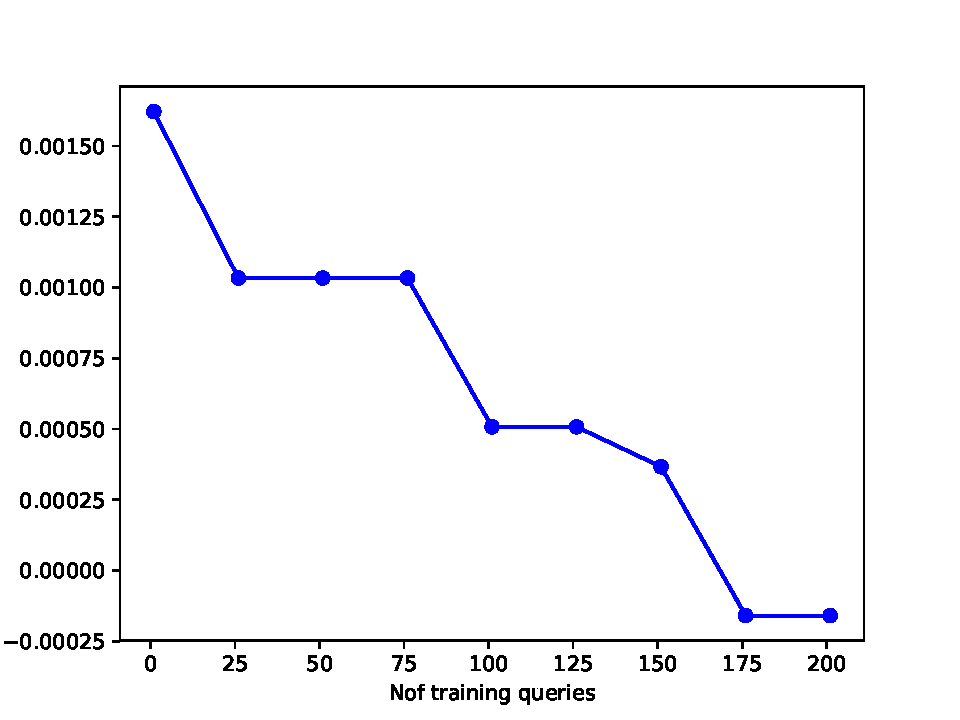
\includegraphics[width=1.0\textwidth]{../figs/tpch10/tpch10_q06_memerror.pdf}
		\caption{Relative Memory Error for query 6}
  \end{figure}
\end{frame}


\begin{frame}[fragile]
	\frametitle{Tpch sf10}
  \begin{figure}[t]
    \centering
    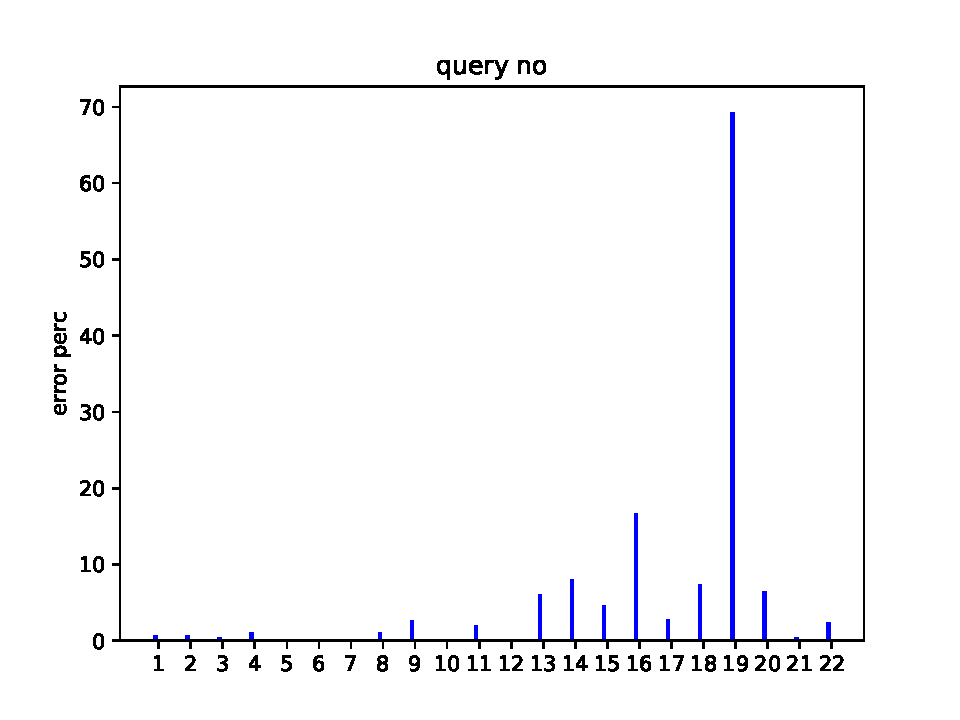
\includegraphics[width=1.0\textwidth]{../figs/tpch10/mem_error_1-23.pdf}
  \end{figure}
\end{frame}

\begin{frame}[fragile]
\frametitle{Airtraffic benchmark suite}
\begin{lstlisting}[basicstyle=\ttfamily\footnotesize, language=SQL,escapechar=!]
SELECT SQL_MIN("Origin", "Dest"),
       SQL_MAX("Origin", "Dest") AS route,
       COUNT(*) AS cnt_before
FROM ontime
!\colorbox{yellow}{WHERE 2010-09-11<FlightDate AND FlightDate<2011-09-11}!
GROUP BY route;
\end{lstlisting}
	\begin{figure}[!htb]
	  \begin{subfigure}[t]{0.5\textwidth}
	    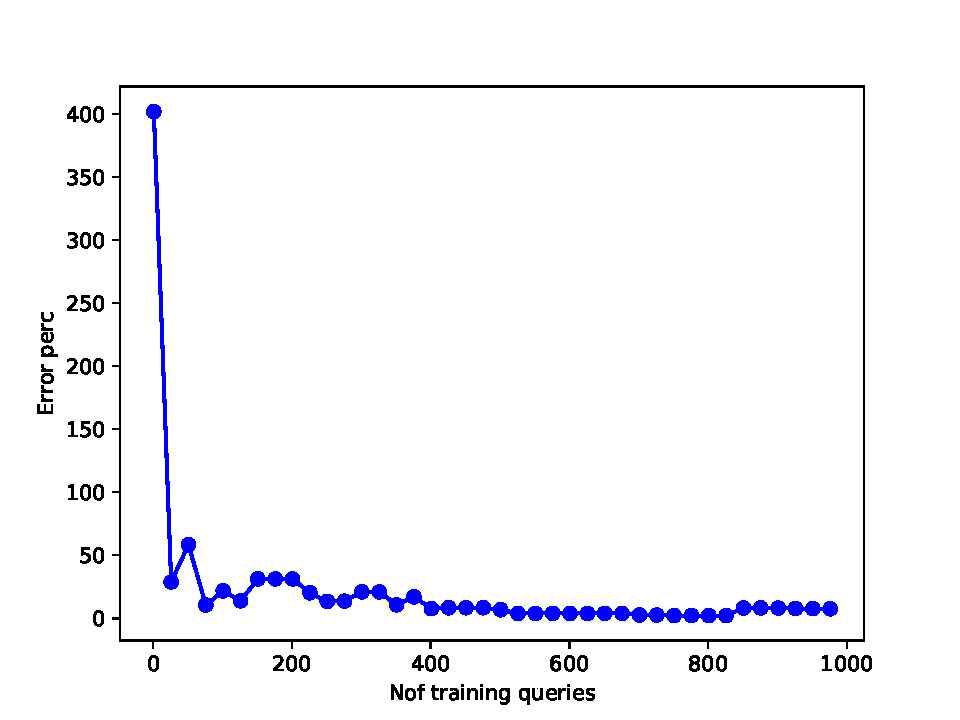
\includegraphics[scale=0.4]{../figs/airtraffic/airtraffic_sel11_error.pdf}
	    \caption{Q11 select error}
	    \label{fig:sel04}
	  \end{subfigure}
	  % \begin{subfigure}[t]{0.4\textwidth}
	  %   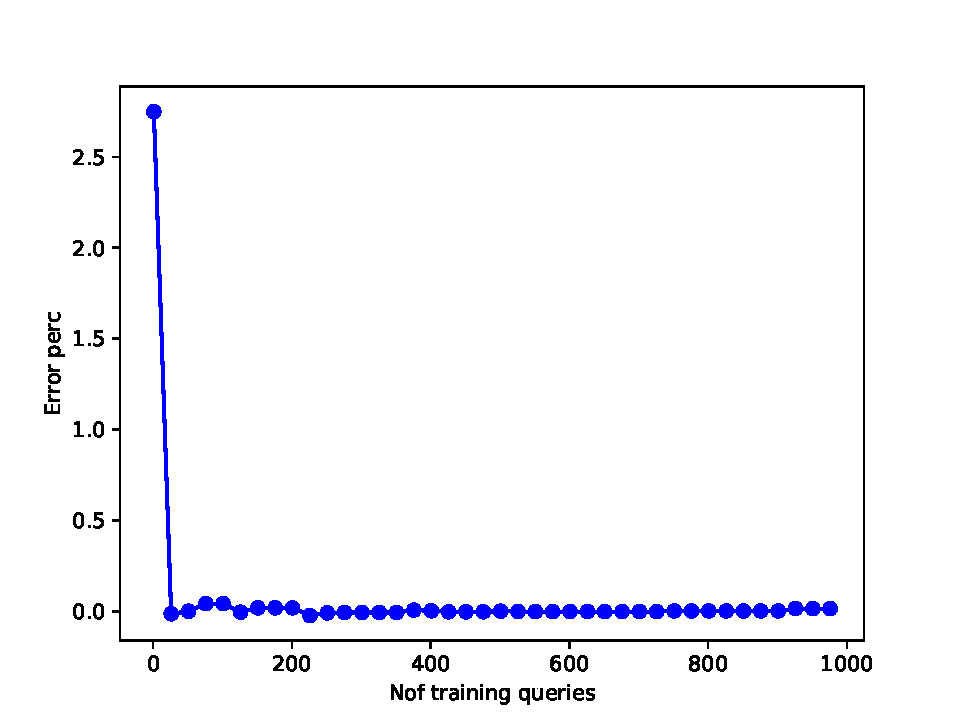
\includegraphics[scale=0.3]{../figs/airtraffic/airtraffic_q11_memerror.pdf}
	  %   \caption{Q11 memory error}
	  %   \label{fig:mem04}
	  %  \end{subfigure}
	\end{figure}
\end{frame}

\begin{frame}[fragile]
\frametitle{Airtraffic benchmark suite}
\begin{lstlisting}[basicstyle=\ttfamily\footnotesize, language=SQL,escapechar=!]
--Query 4
SELECT "DayOfWeek", COUNT(*) AS "Flights"
FROM ontime
!\colorbox{yellow}{WHERE "DepDelay" > 15}!
GROUP BY "DayOfWeek"
ORDER BY "DayOfWeek";
\end{lstlisting}
	\begin{figure}[!htb]
	  % \begin{subfigure}[t]{0.4\textwidth}
	  %   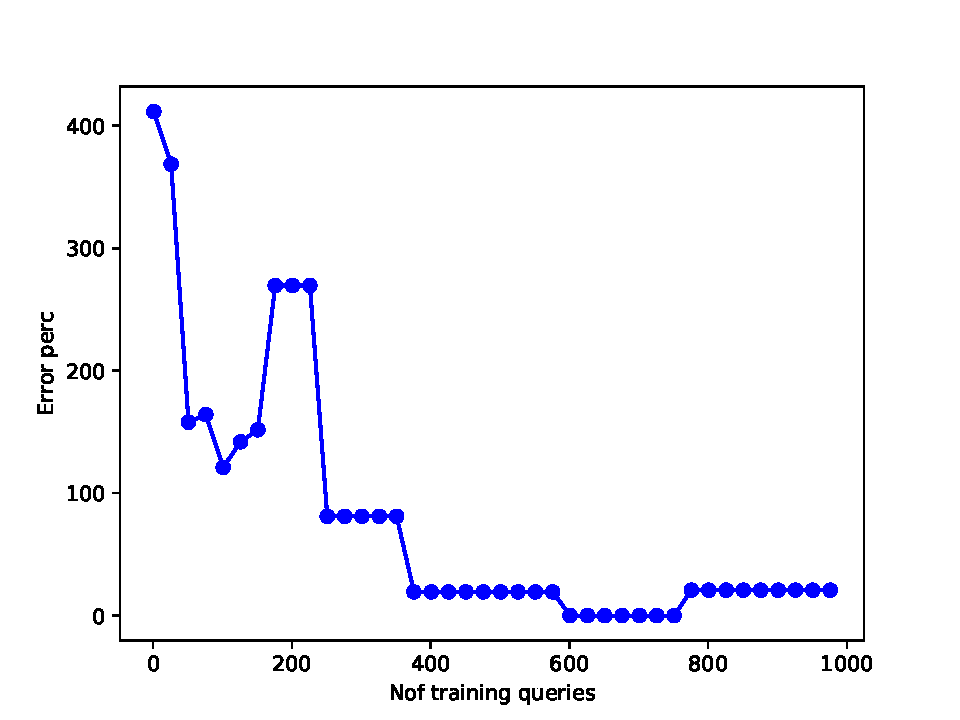
\includegraphics[scale=0.3]{../figs/airtraffic/airtraffic_sel04_error.pdf}
	  %   \caption{Q04 select error}
	  %   \label{fig:sel04}
	  % \end{subfigure}
	  % \begin{subfigure}[t]{0.4\textwidth}
		\centering
	  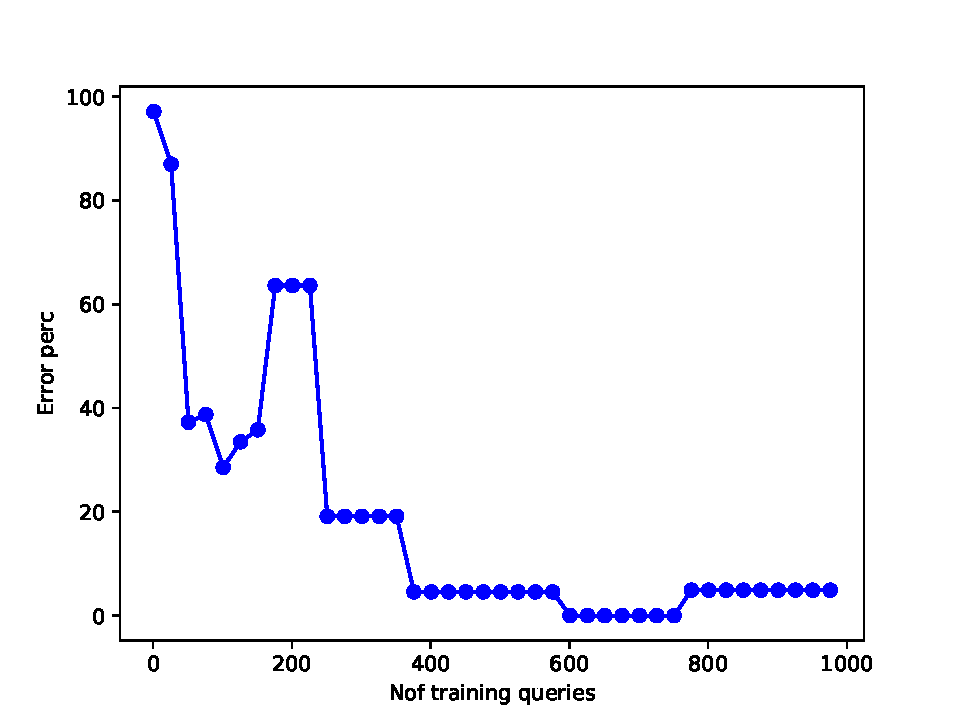
\includegraphics[scale=0.4]{../figs/airtraffic/airtraffic_q04_memerror.pdf}
	  \caption{Q04 memory error}
	    \label{fig:mem04}
	  %  \end{subfigure}
	\end{figure}
\end{frame}


\begin{frame}[fragile]
\frametitle{Airtraffic benchmark suite}
\begin{lstlisting}[basicstyle=\ttfamily\footnotesize, language=SQL, escapechar=!]
SELECT "Origin" AS ap, COUNT(*) AS cnt_in
FROM ontime
!\colorbox{yellow}{WHERE "Dest" = 'ORD'}!
GROUP BY "Origin"
\end{lstlisting}
	\begin{figure}[!htb]
	  \begin{subfigure}[t]{0.5\textwidth}
	    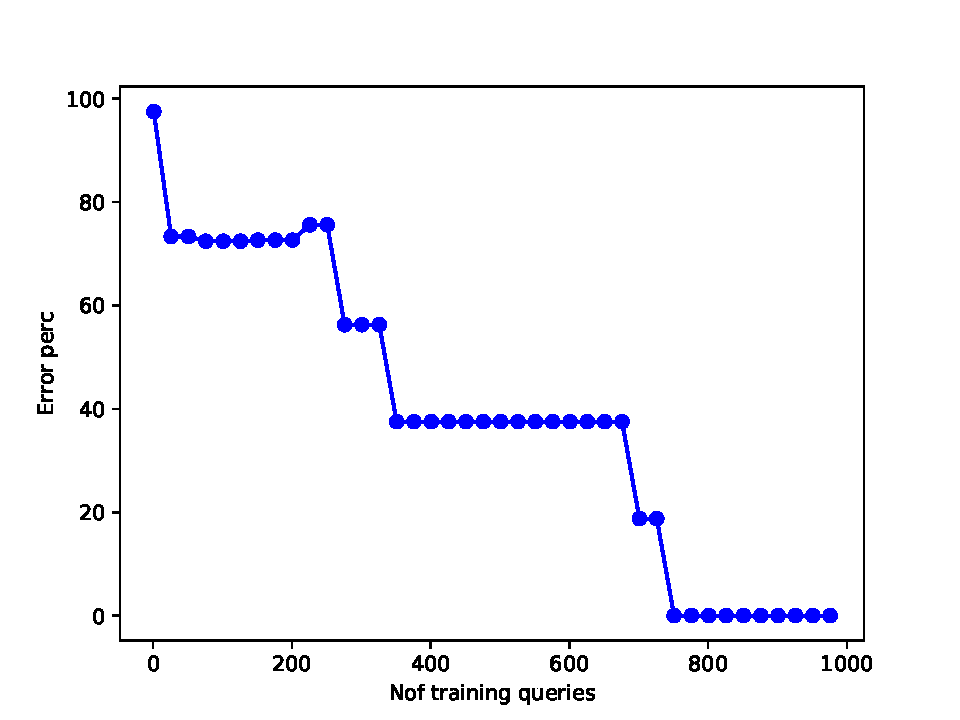
\includegraphics[scale=0.4]{../figs/airtraffic/airtraffic_sel10_error.pdf}
	    \caption{Q10 select error}
	    \label{fig:sel04}
	  \end{subfigure}
	  % \begin{subfigure}[t]{0.4\textwidth}
	  %   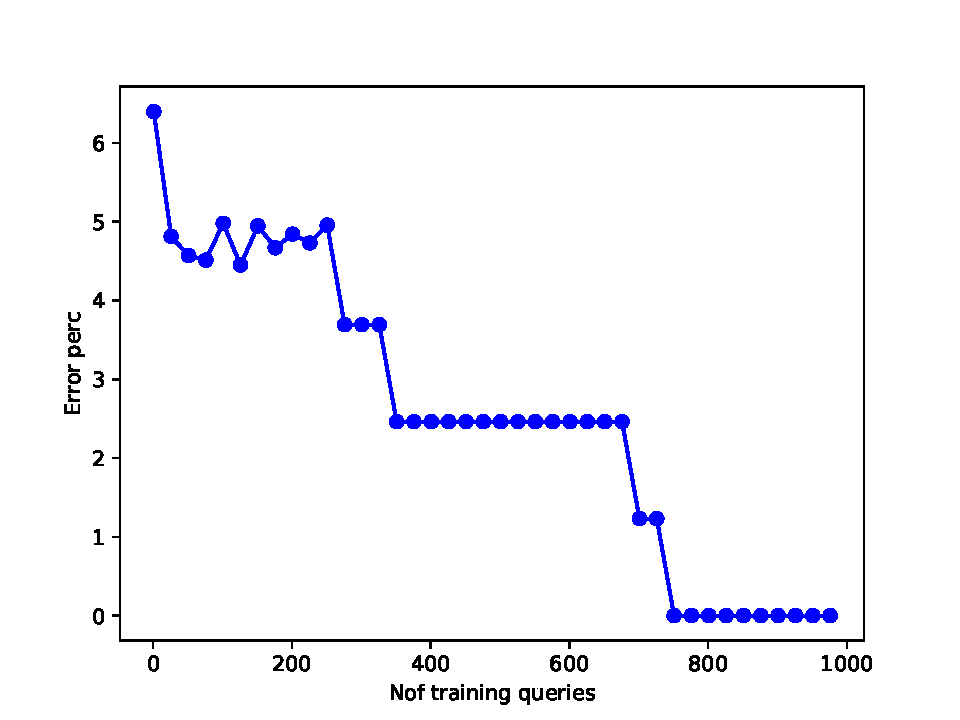
\includegraphics[scale=0.3]{../figs/airtraffic/airtraffic_q10_memerror.pdf}
	  %   \caption{Q10 memory error}
	  %   \label{fig:mem04}
	  %  \end{subfigure}
	\end{figure}
\end{frame}

\begin{frame}[fragile]
\frametitle{Airtraffic benchmark suite}
\begin{lstlisting}[basicstyle=\ttfamily\footnotesize, language=SQL, escapechar=!]
SELECT *
FROM ontime
!\colorbox{yellow}{WHERE "DepDelay" > 15 AND "ArrDelay" > 15}!
!\colorbox{yellow}{AND "Month" = 3 AND "DayofMonth" = 24 AND "Year" = 2013}!
\end{lstlisting}
	\begin{figure}[!htb]
	  \begin{subfigure}[t]{0.5\textwidth}
	    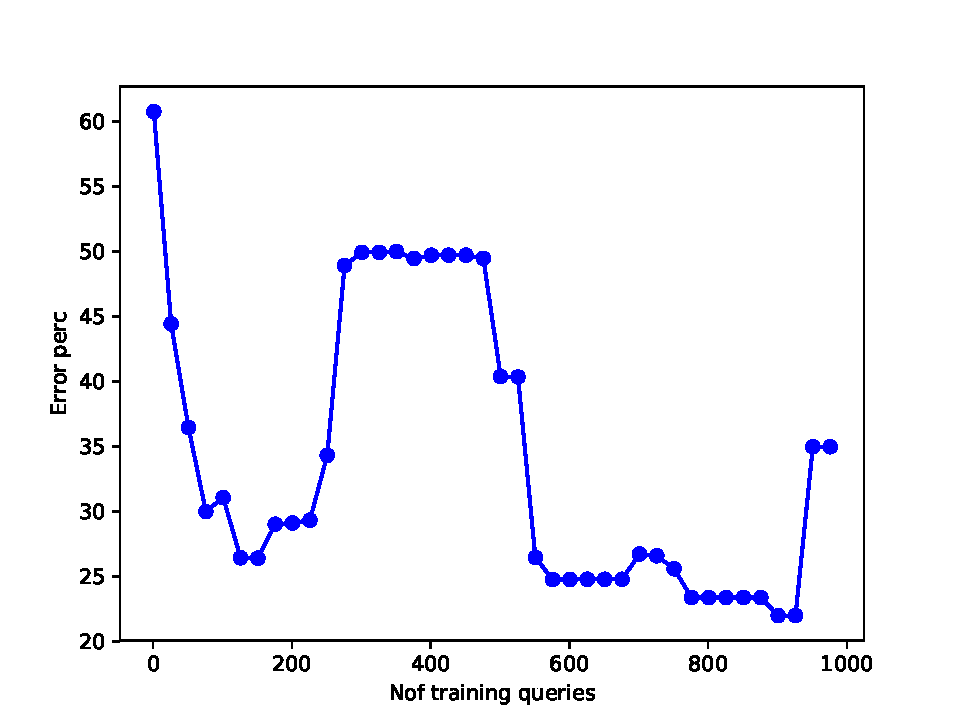
\includegraphics[scale=0.4]{../figs/airtraffic/airtraffic_sel09_error.pdf}
	    \caption{Q09 select error}
	    \label{fig:sel04}
	  \end{subfigure}
	  % \begin{subfigure}[t]{0.4\textwidth}
	  %   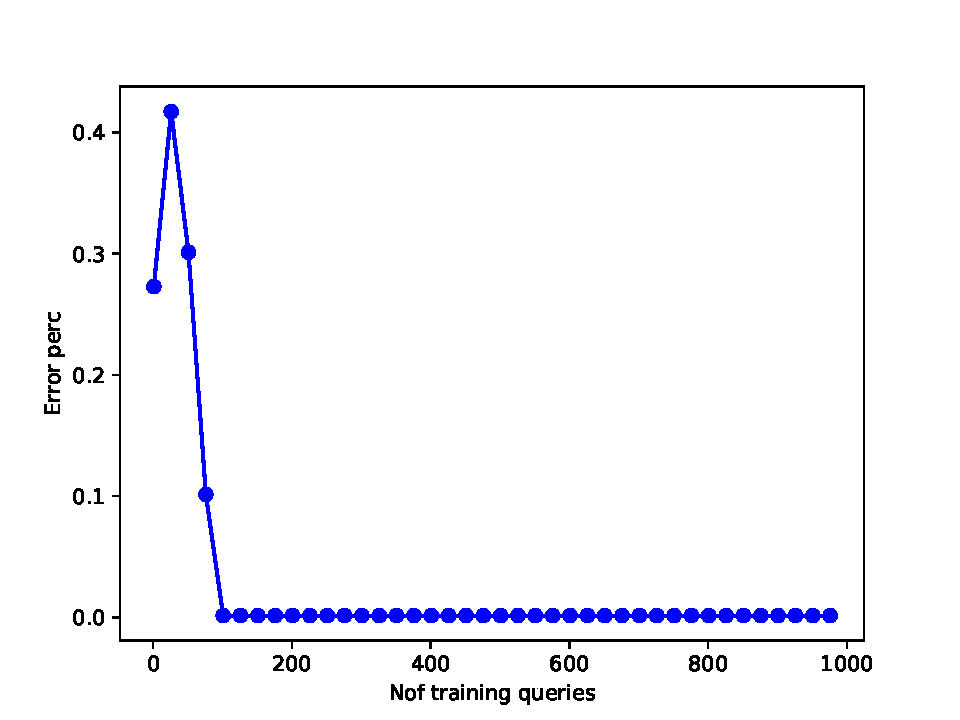
\includegraphics[scale=0.3]{../figs/airtraffic/airtraffic_q09_memerror.pdf}
	  %   \caption{Q09 memory error}
	  %   \label{fig:mem04}
	  %  \end{subfigure}
	\end{figure}
\end{frame}


\begin{frame}[fragile]
\frametitle{Future Work}
\begin{block}{}
\begin{itemize}
\item Provide min,avg,max policies
\item Consider parallel executions
\item Also use histograms
\end{itemize}
\end{block}
\end{frame}
